\documentclass[tikz,border=1mm]{standalone}
\usetikzlibrary{matrix,chains,positioning,decorations.pathreplacing,arrows,shapes.geometric}

\begin{document}
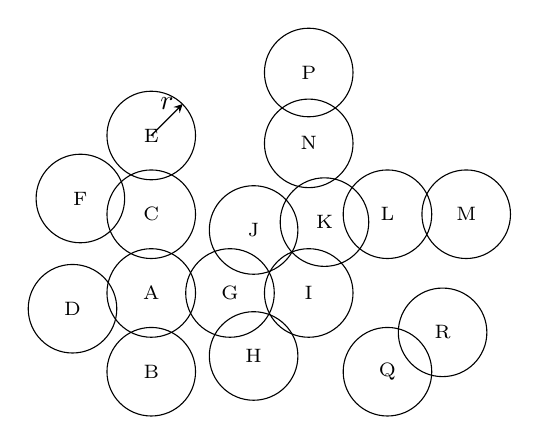
\begin{tikzpicture}[>=latex]
\foreach \x/\y/\name in 
    % {0/0/A, 
    %  1/1/B,
    %  2/2/C,
    %  0/-1/D,
    %  -1.5/-1/E,
    %  0.75/-.5/F,
    %  -0.6/0.8/G,
    %  1-0.2/-2/H,
    %  2/-1/L,
    %  3/3/I,
    %  3/1.7/J,
    %  3/1-.4/K
    %  }
    {
     0/0/A,
    -0/-1/B,
    0/1/C,
    -1/-0.2/D,
    1/0/G,
    -.9/1.2/F,
    0/2/E,
    1.3/-0.8/H,
    1.3/0.8/J,
    2/0/I,
    2.2/.9/K,
    3/1/L,
    4/1/M,
    2/1.9/N,
    2/2.8/P, 
    % 2.9/2.3/O,
    3/-1/Q,
    3.7/-0.5/R
    %  -1.8/0/E,
    %  -1.8/-1.8/F,
    %  1.8/-1.8/G,
    %  0.8/-1.8/H,
    %  2/-0.5/I,
    %  2/0.5/J,
    %  1/1/K,
    %  2/2/L,
    %  3/3/M,
    %  4/5/N,
    %  4/3/O,
    %  4/2/P,
    %  5/4/Q,
    %  6/4/R, 
    %  1/4/S,
    %  2/5/T,
    }
    {
    \draw (\x,\y) circle(16pt) node {\scriptsize\name};
    % \draw (\x,\y) circle(5pt) ;
    
    }

\draw[-stealth] (0,2) -- (.4,2.4) node [midway, above] {$r$};

% \draw[step=1,gray] (-2,-2) grid (12,12);
% \foreach \x in {0,1,2,3,4,5,6,7,8,9,10}
%    \draw (\x cm,1pt) -- (\x cm,-1pt) node[anchor=north] {$\x$};
% \foreach \y in {0,1,2,3,4,5,6,7,8,9,10}
%     \draw (1pt,\y cm) -- (-1pt,\y cm) node[anchor=east] {$\y$};



\end{tikzpicture}
\end{document}
